%!TEX root = matmul_wse.tex

\subsection{Block instead of Vector}

If using block instead of vector, then the number of iteration is $PE_x$ instead of $K$.
%
Therefore, if still considering the top right corner PE and FP16, in each iteration, the number cycles of FMAC is: $MB * NB * KB / 4$; while it needs $PE_x+MB \times KB/4$ cycles to receive $A$ (activation) and $PE_y+NB \times KB/2$ cycles to receive $B$ (weight).


In this case, Equation~\ref{eq:summa_1} becomes:
\begin{equation}
  MB \times NB \times KB/(MB \times NB \times KB +4 \times PE_x + 2 \times MB \times KB+4 \times PE_y + 2 \times NB \times KB)
  \label{eq:summa_4}
\end{equation}
%
Equation~\ref{eq:summa_2} becomes:
\begin{equation}
  MB \times NB \times KB/(MB \times NB \times KB +max(4 \times PE_x + 2 \times MB \times KB, 4 \times PE_y + 2 \times NB \times KB))
  \label{eq:summa_5}
\end{equation}
%
Equation~\ref{eq:summa_3} becomes:
\begin{equation}
  MB \times NB \times KB/max(MB \times NB \times KB, 4 \times PE_x + 2 \times MB \times KB, 4 \times PE_y + 2 \times NB \times KB)
  \label{eq:summa_6}
\end{equation}

This way relaxes the urgency of the communication and creates more rooms to overlap communication and computation, and Fig.~\ref{fig:gemm_perf_simulate_block} updates Fig.~\ref{fig:gemm_perf_simulate} with this optimization, which is called ``BLOCK'' instead of ``VECTOR''.


\begin{figure}[t!]
  \centering
  \begin{subfigure}{0.32\columnwidth}
    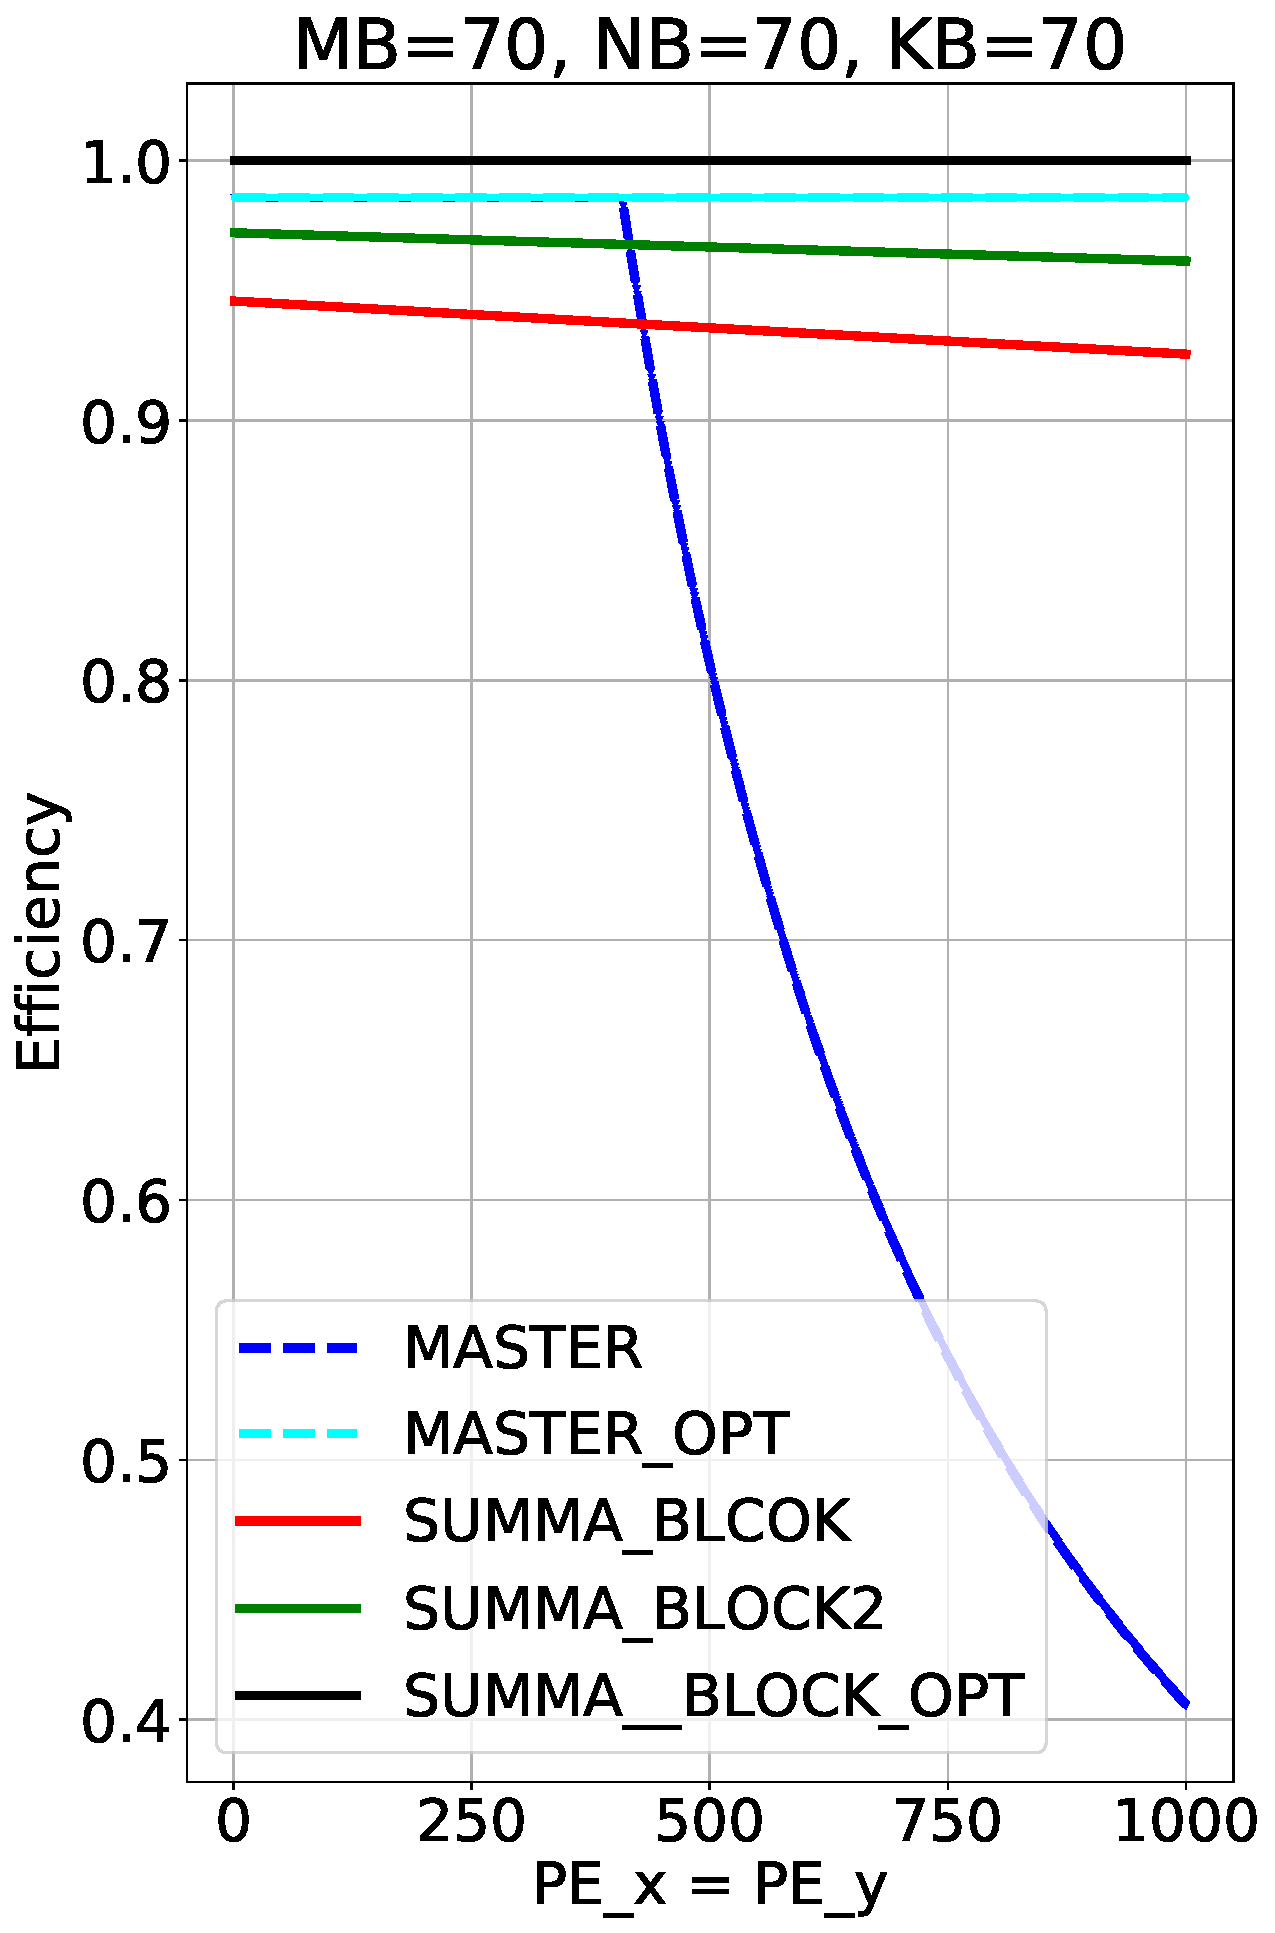
\includegraphics[width=\linewidth]{figures/efficiency_cost_block_70_70_70.pdf}
    %\caption{.}
    %\label{fig:gemm_master_1}
  \end{subfigure}
  \hfill
  %
  \begin{subfigure}{0.32\columnwidth}
    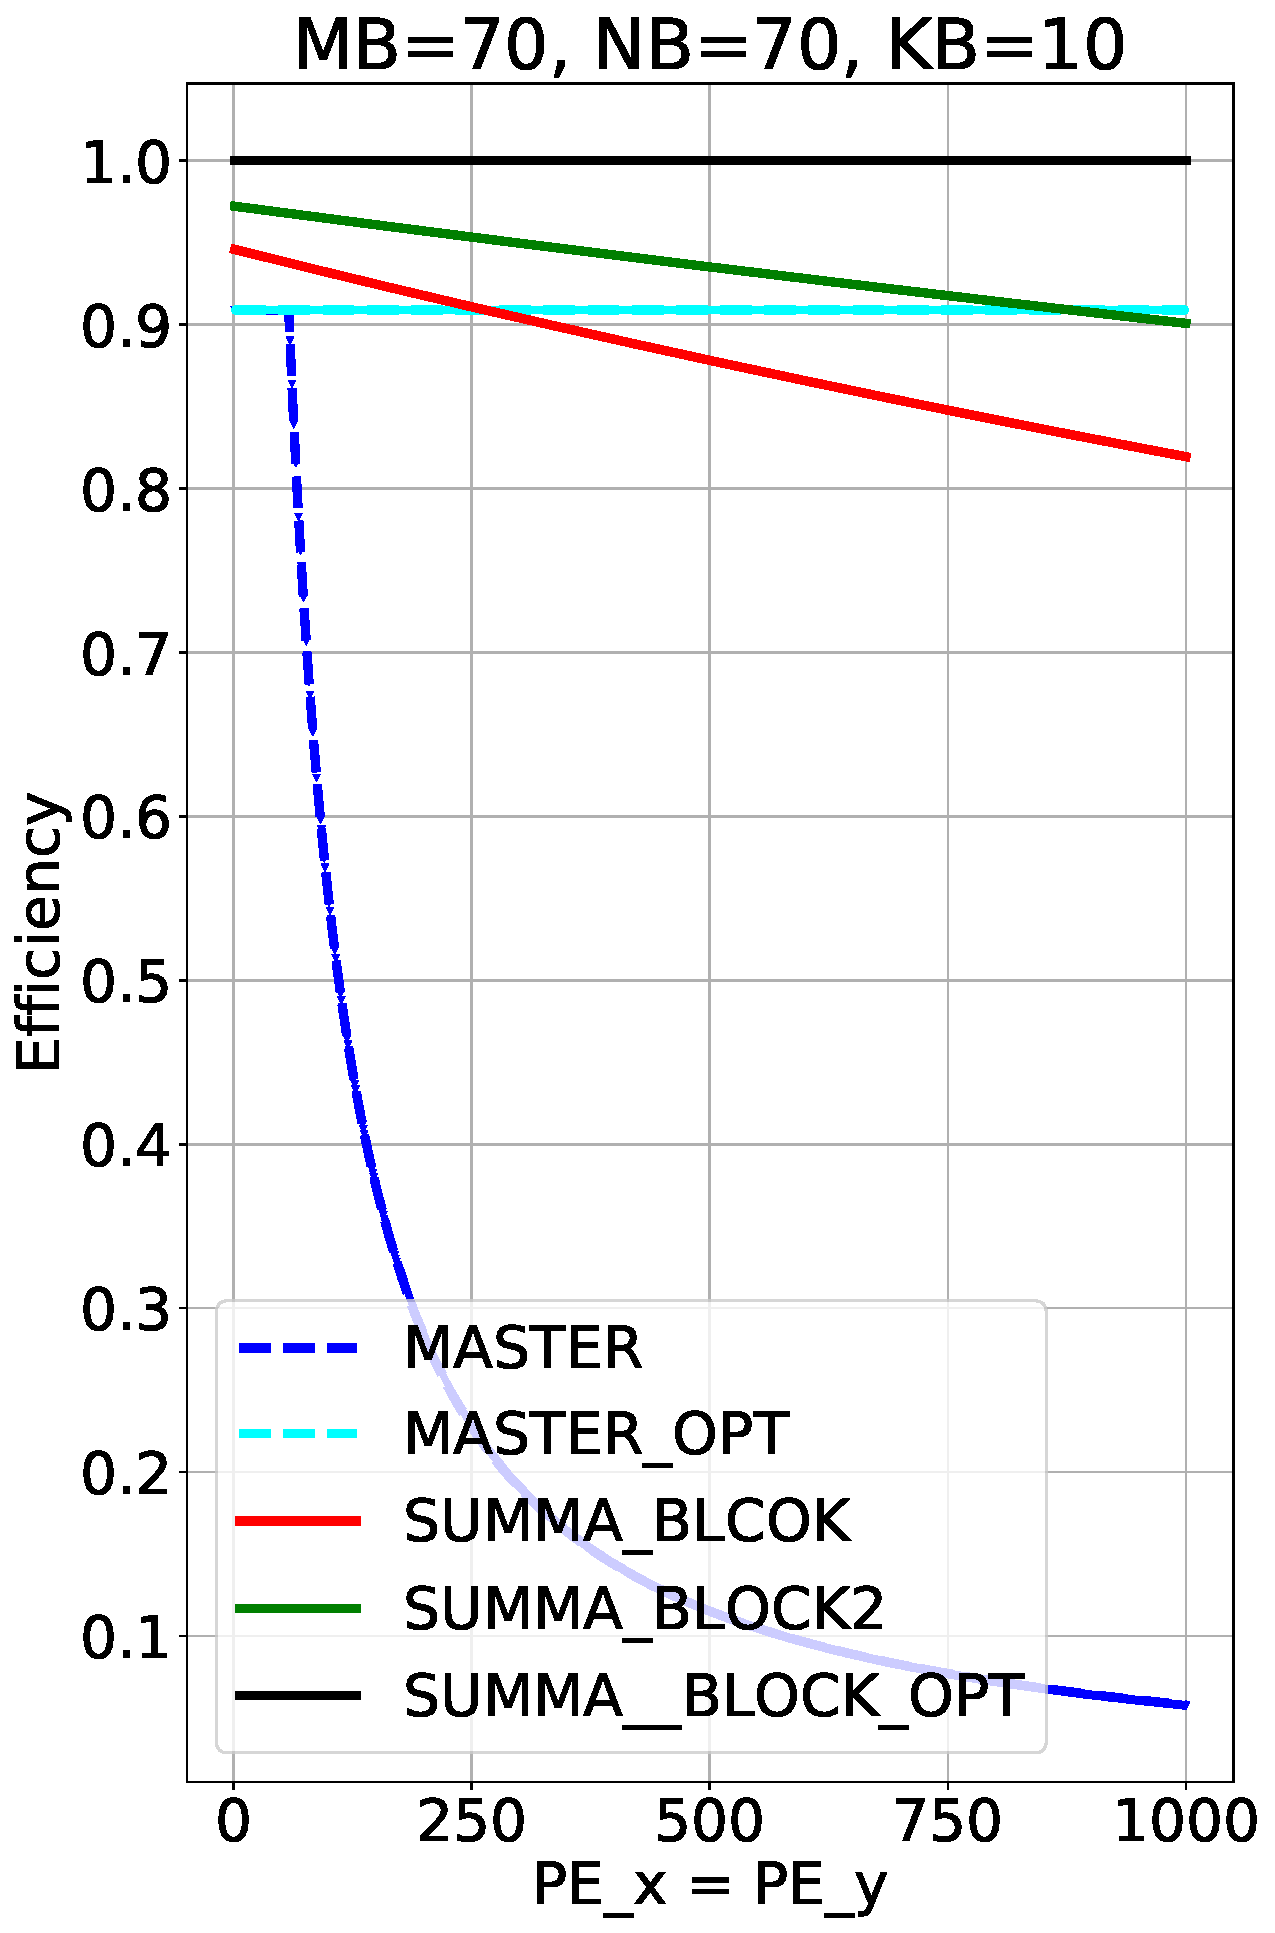
\includegraphics[width=\linewidth]{figures/efficiency_cost_block_70_70_10.pdf}
    %\caption{Non-ring.}
    %\label{fig:gemm_master_2}
  \end{subfigure}
  \hfill
  %
  \begin{subfigure}{0.32\columnwidth}
    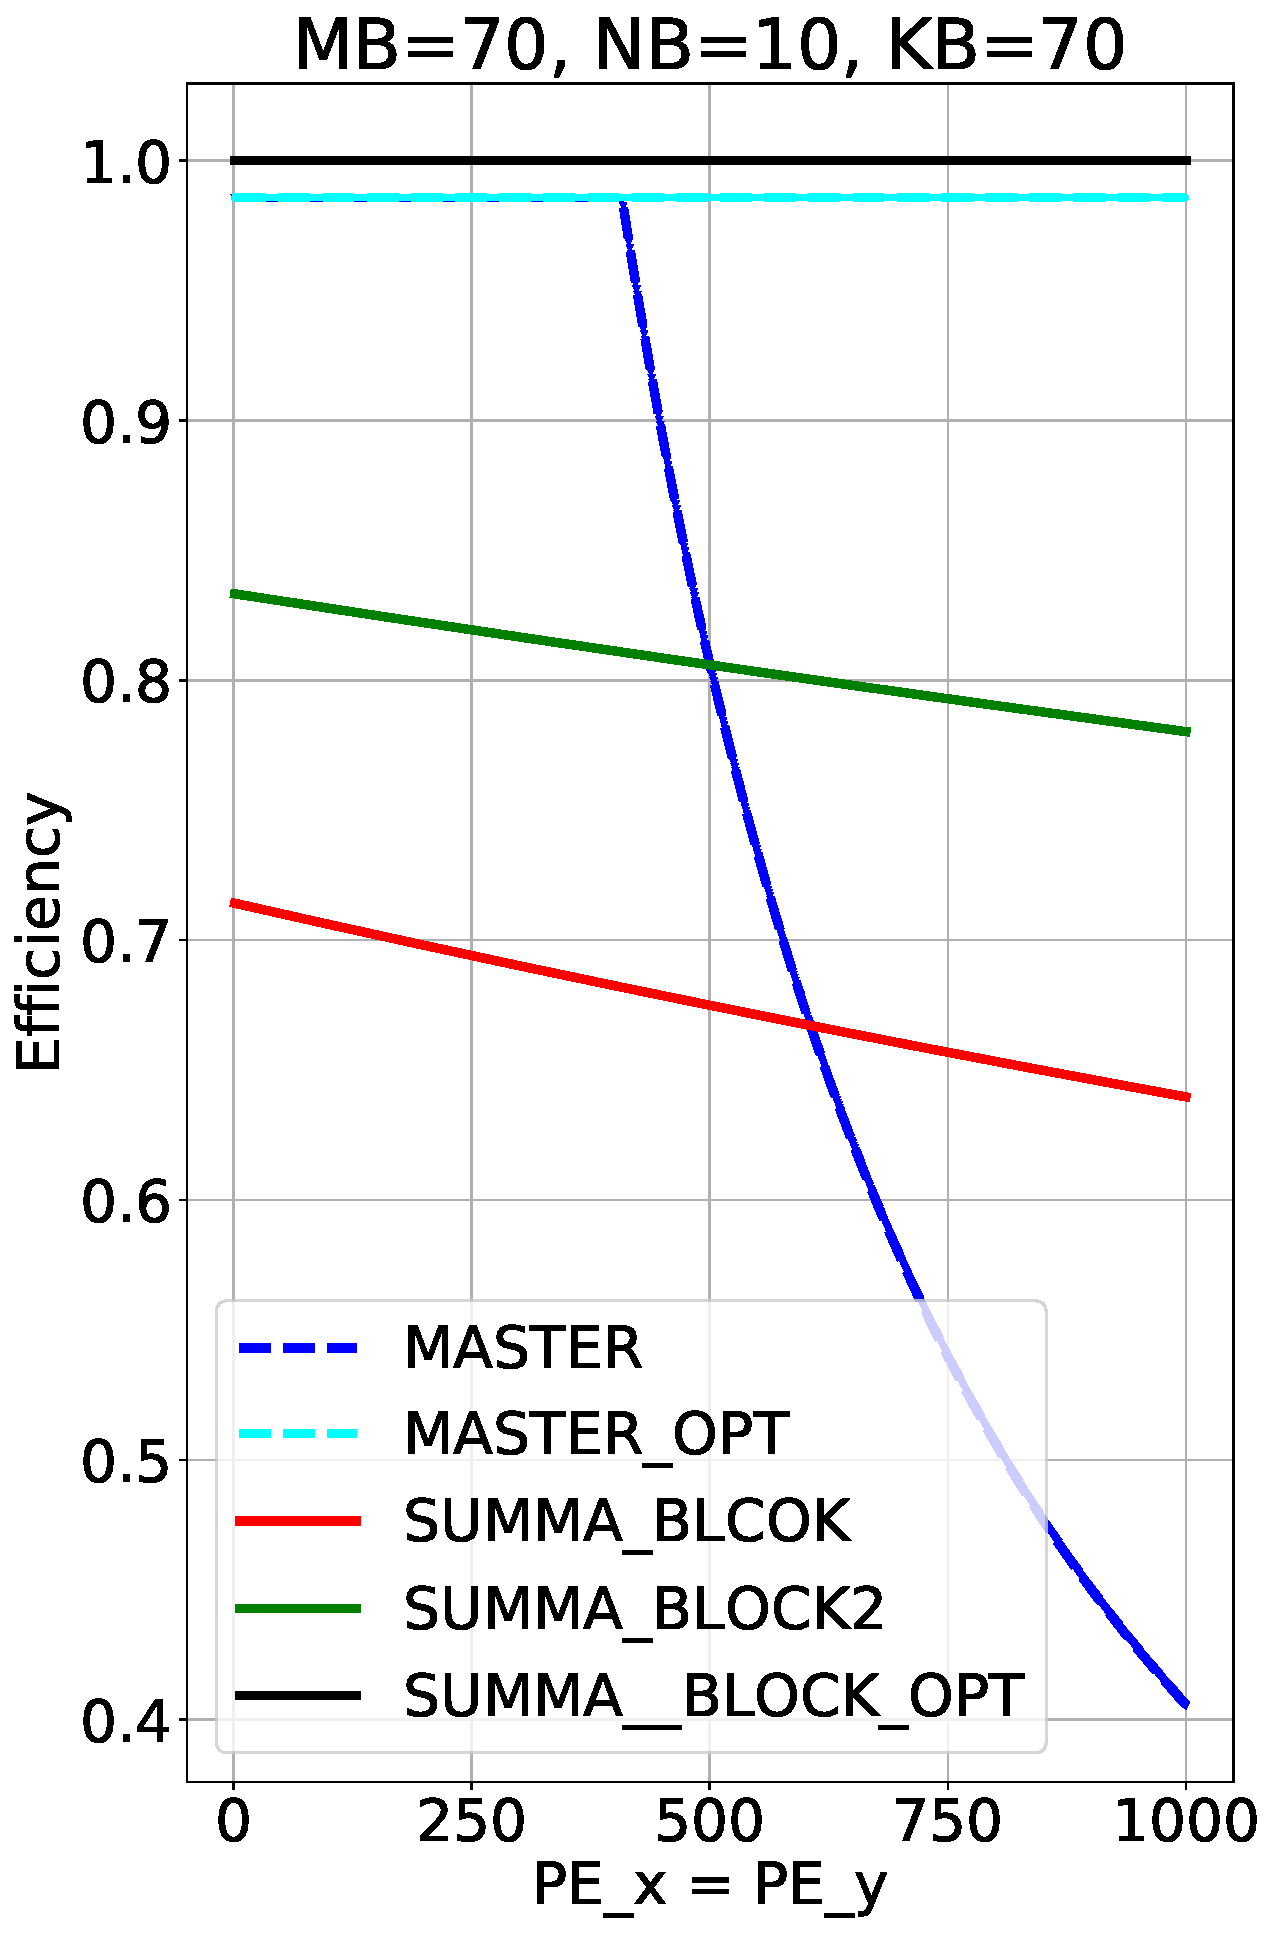
\includegraphics[width=\linewidth]{figures/efficiency_cost_block_70_10_70.pdf}
    %\caption{Non-ring.}
    %\label{fig:gemm_master_2}
  \end{subfigure}
  \caption{Performance simulation. ``MASTER": Equation~\ref{eq:master}; ``MASTER\_OPT": Equation~\ref{eq:master_2}; ``SUMMA\_BLOCK'': Equation~\ref{eq:summa_4}; ``SUMMA\_BLOCK2'': Equation~\ref{eq:summa_5}; ``SUMMA\_BLOCK\_OPT'': Equation~\ref{eq:summa_6}.}
  \label{fig:gemm_perf_simulate_block}
\end{figure}
 

%\subsection{Overlap Computation and Communication?}


%\subsection{FIFO??}


\subsection{Ideal}


The ideal \summa should be (1) communication perfectly by computation (2) pipelined.
%
Therefore, the total number of cycles for a MatMul problem on FP16 is $max(MB \times NB \times K / 4, PE_x + MB \times K/2,  PE_y + NB \times K/2)$:
Equation~\ref{eq:summa_3} becomes:
\begin{equation}
  MB \times NB \times K/max(MB \times NB \times K, 4 \times PE_x + 2 \times MB \times K, 4 \times PE_y + 2 \times NB \times K)
  \label{eq:summa_7}
\end{equation}
%
Fig.~\ref{fig:gemm_perf_simulate_ideal} mimics three scenarios of square matrices with relative small sizes.
%
{\bf However, this is the ideal, and I'm not sure whether it's achievable or not.}


\begin{figure}[t!]
  \centering
  \begin{subfigure}{0.32\columnwidth}
    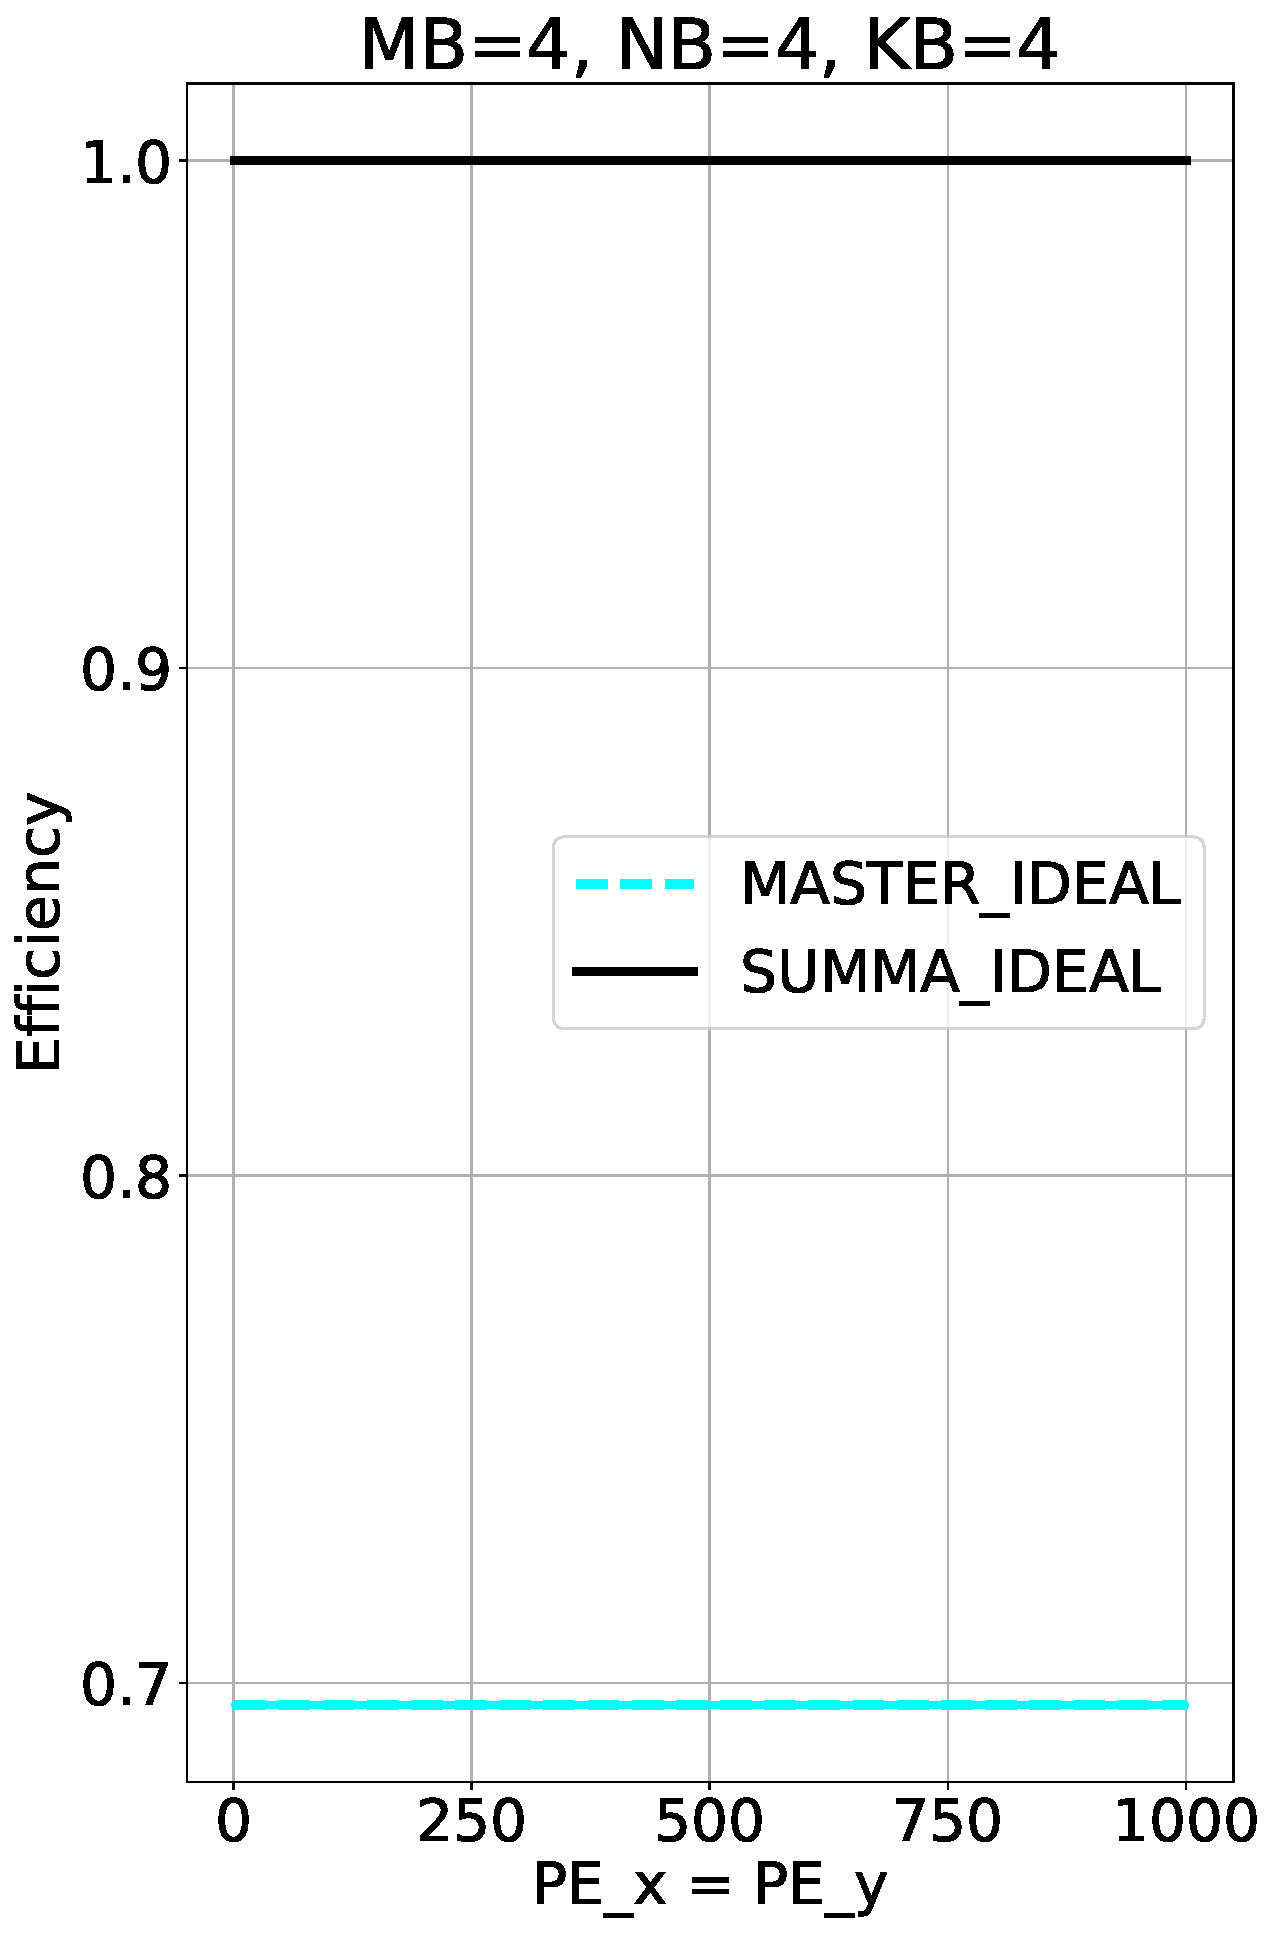
\includegraphics[width=\linewidth]{figures/efficiency_cost_ideal_4_4_4.pdf}
    %\caption{.}
    %\label{fig:gemm_master_1}
  \end{subfigure}
  \hfill
  %
  \begin{subfigure}{0.32\columnwidth}
    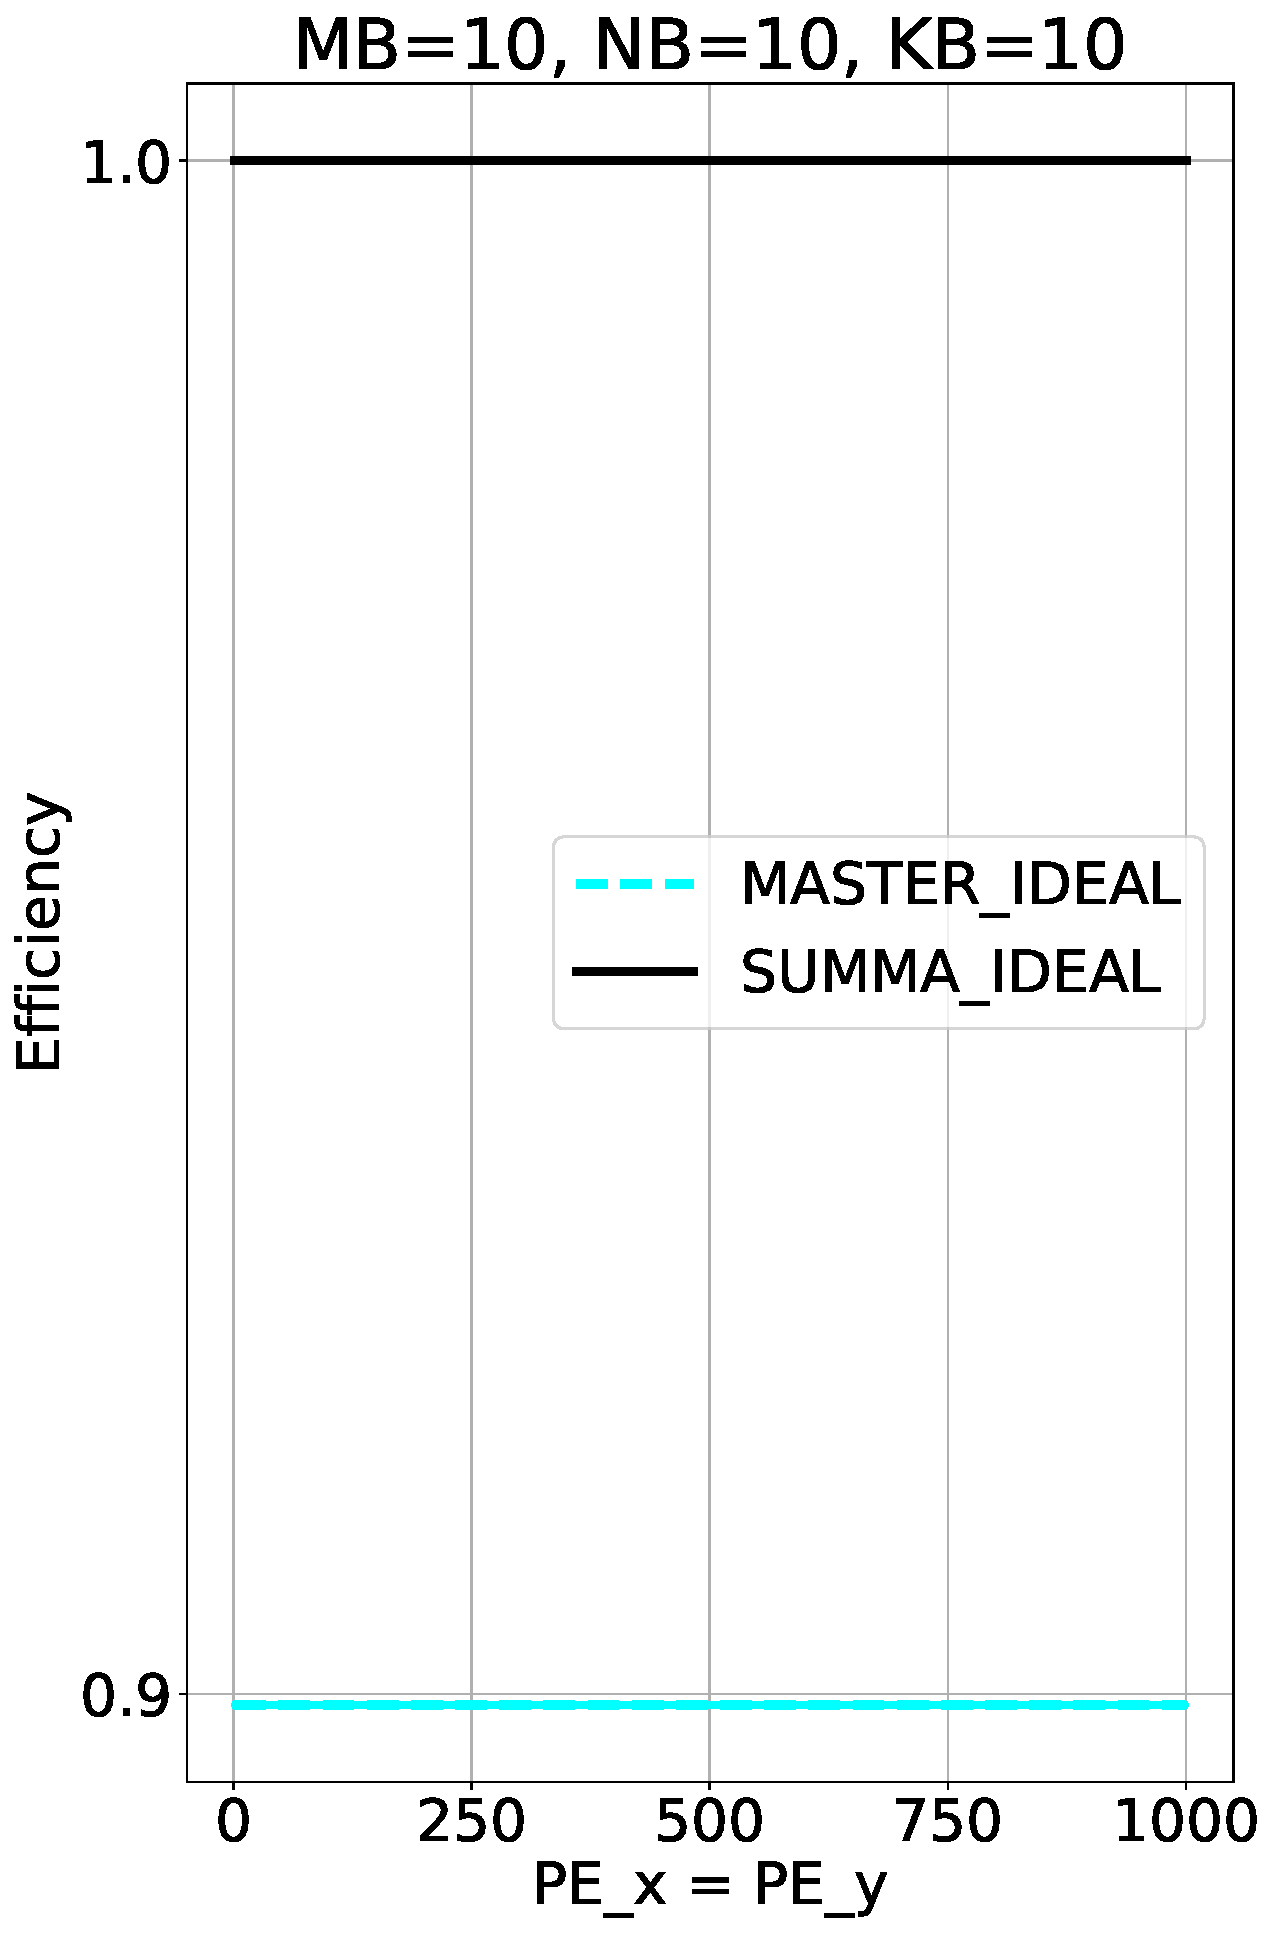
\includegraphics[width=\linewidth]{figures/efficiency_cost_ideal_10_10_10.pdf}
    %\caption{Non-ring.}
    %\label{fig:gemm_master_2}
  \end{subfigure}
  \hfill
  %
  \begin{subfigure}{0.32\columnwidth}
    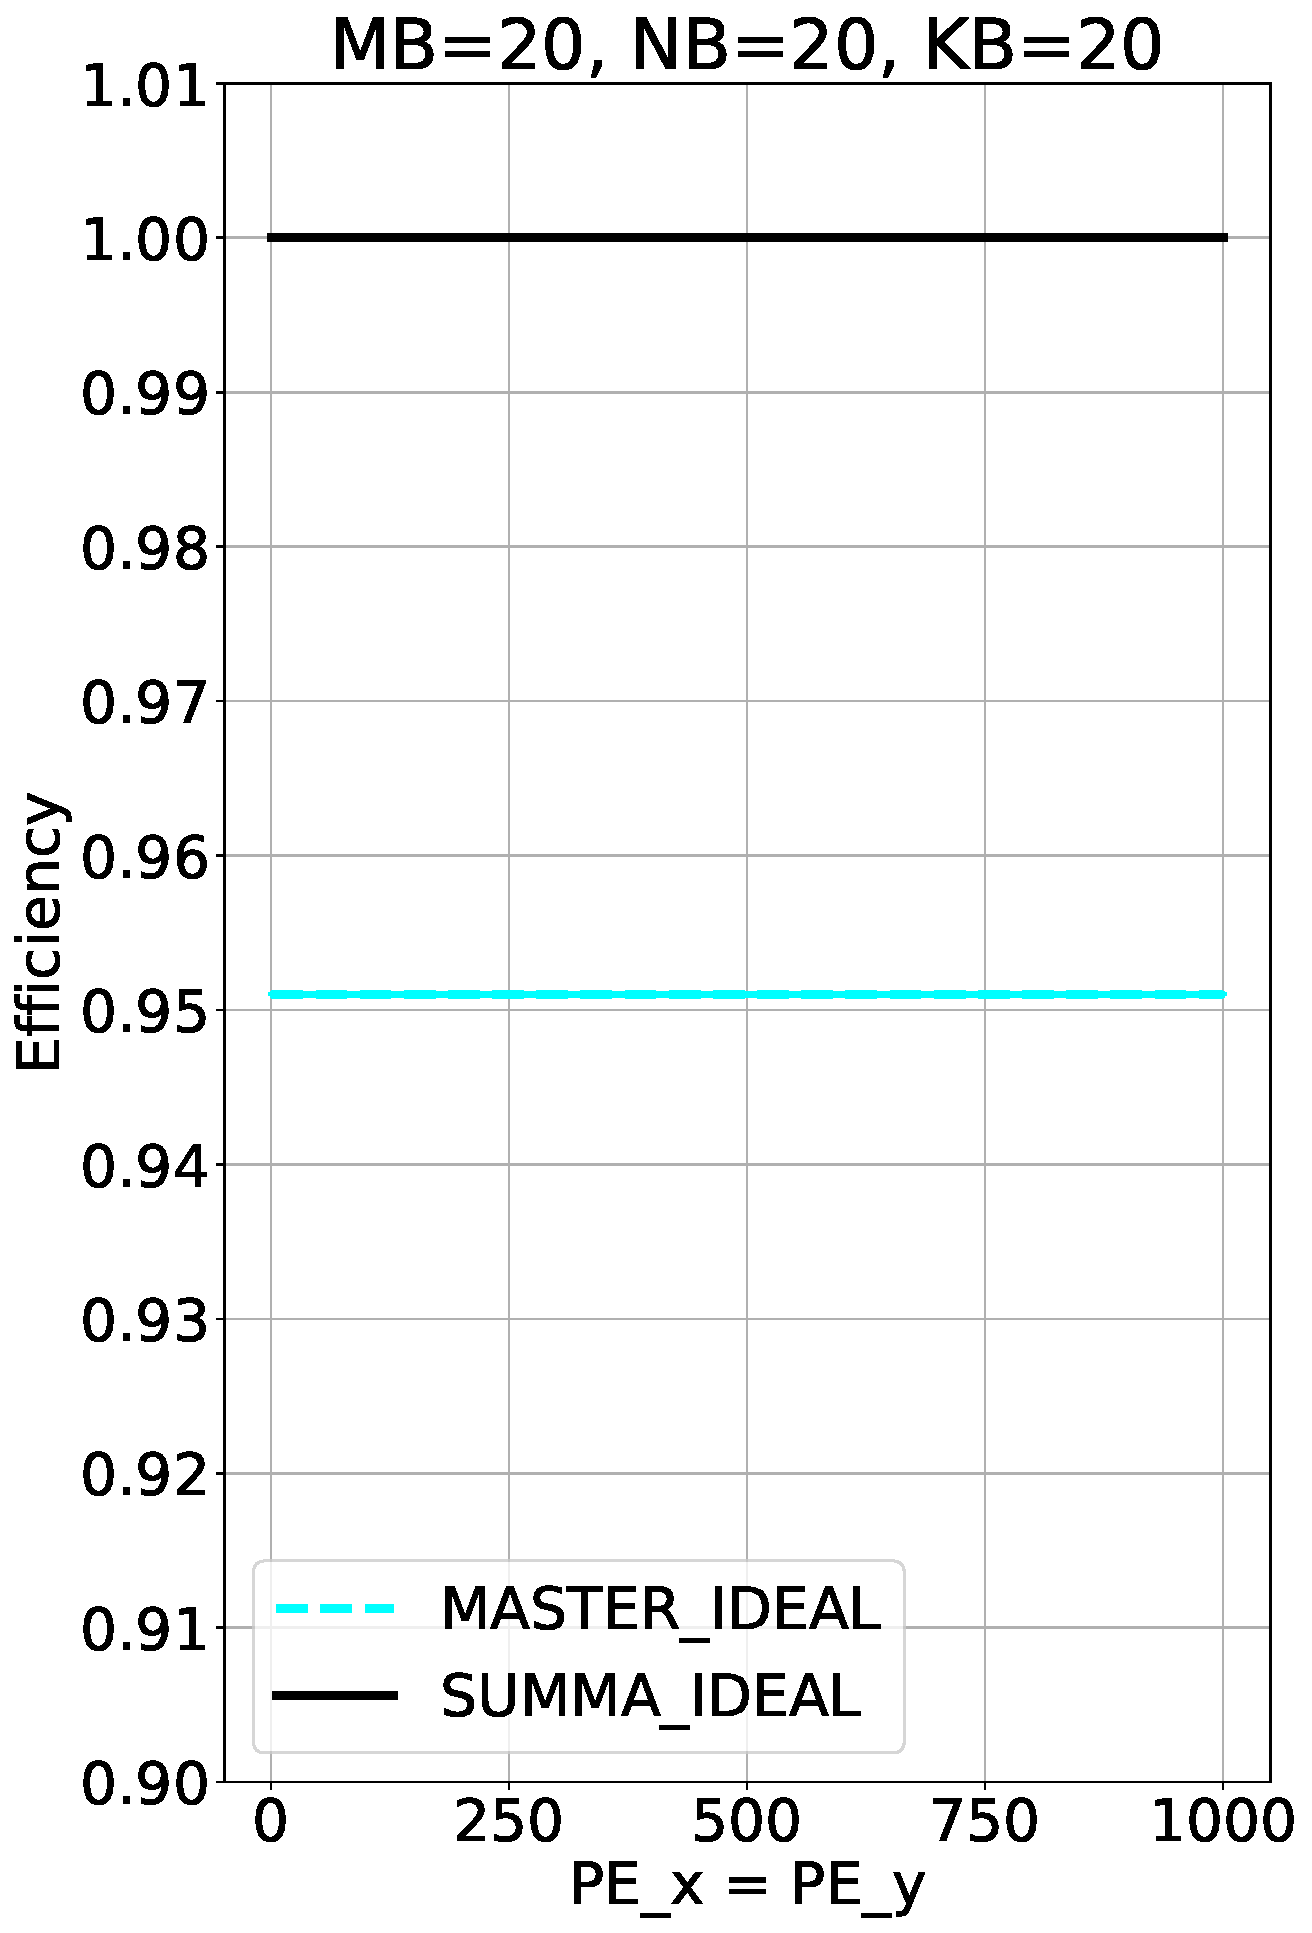
\includegraphics[width=\linewidth]{figures/efficiency_cost_ideal_20_20_20.pdf}
    %\caption{Non-ring.}
    %\label{fig:gemm_master_2}
  \end{subfigure}
  \caption{Performance simulation. ``MASTER\_IDEAL": Equation~\ref{eq:master_2}; ``SUMMA\_IDEAL'': Equation~\ref{eq:summa_7}.}
  \label{fig:gemm_perf_simulate_ideal}
\end{figure}




